\documentclass[10pt,a4paper]{article}
\usepackage[margin=18mm,includeheadfoot]{geometry}
\usepackage{fontspec}
\setmainfont{Noto Serif}
\setsansfont{Noto Sans}
\setmonofont{Noto Sans Mono}
\usepackage{amsmath,amssymb,amsthm,mathtools}
\usepackage{graphicx}
\setkeys{Gin}{keepaspectratio}
\usepackage{booktabs,longtable,array,tabularx}
\usepackage{microtype}
\usepackage{enumitem}
\usepackage{xcolor}
\usepackage{hyperref}
\usepackage{bookmark}
\usepackage{fancyvrb}
\usepackage{fvextra}
\usepackage{upquote}
\usepackage{csquotes}
\usepackage{caption}
\usepackage{float}
\usepackage{fancyhdr}
\usepackage{lastpage}
\usepackage{titlesec}
\usepackage{setspace}
\usepackage{etoolbox}
\usepackage{url}
\usepackage{multirow}
\usepackage{makecell}
\hypersetup{colorlinks=true,linkcolor=black,citecolor=black,urlcolor=blue,pdfauthor={Anonymous submission draft},pdftitle={Phase
Erasure Can Hide Agreement-Violation Witnesses in Certificate-Driven
Locking BFT Protocols}}
\setlist{nosep,leftmargin=*}
\setlength{\parindent}{1em}
\setlength{\parskip}{0.25em}
\setlength{\emergencystretch}{2em}
\captionsetup{font=small,labelfont=bf}
\titleformat{\section}{\large\bfseries}{}{0em}{}
\titleformat{\subsection}{\normalsize\bfseries}{}{0em}{}
\titleformat{\subsubsection}{\normalsize\itshape}{}{0em}{}
\titlespacing*{\section}{0pt}{1.0em}{0.35em}
\titlespacing*{\subsection}{0pt}{0.8em}{0.25em}
\titlespacing*{\subsubsection}{0pt}{0.65em}{0.2em}
\newtheorem{theorem}{Theorem}
\newtheorem{lemma}{Lemma}
\newtheorem{proposition}{Proposition}
\newtheorem{definition}{Definition}
\newcommand{\UnsafeObs}{\mathsf{UnsafeObs}}
\newcommand{\tightlist}{\setlength{\itemsep}{0pt}\setlength{\parskip}{0pt}}
\providecommand{\pandocbounded}[1]{#1}
\NewDocumentCommand\citeproctext{}{}
\NewDocumentCommand\citeproc{mm}{%
  \begingroup\def\citeproctext{#2}\cite{#1}\endgroup}
\makeatletter
\let\@cite@ofmt\@firstofone
\def\@biblabel#1{}
\def\@cite#1#2{{#1\if@tempswa , #2\fi}}
\makeatother
\newlength{\cslhangindent}
\setlength{\cslhangindent}{1.5em}
\newlength{\csllabelwidth}
\setlength{\csllabelwidth}{3em}
\newenvironment{CSLReferences}[2]
 {\begin{list}{}{%
  \setlength{\itemindent}{0pt}
  \setlength{\leftmargin}{0pt}
  \setlength{\parsep}{0pt}
  \ifodd #1
   \setlength{\leftmargin}{\cslhangindent}
   \setlength{\itemindent}{-1\cslhangindent}
  \fi
  \setlength{\itemsep}{#2\baselineskip}}}
 {\end{list}}
\newcommand{\CSLBlock}[1]{\hfill\break\parbox[t]{\linewidth}{\strut\ignorespaces#1\strut}}
\newcommand{\CSLLeftMargin}[1]{\parbox[t]{\csllabelwidth}{\strut#1\strut}}
\newcommand{\CSLRightInline}[1]{\parbox[t]{\dimexpr\linewidth-\csllabelwidth\relax}{\strut#1\strut}}
\newcommand{\CSLIndent}[1]{\hspace{\cslhangindent}#1}
\pagestyle{fancy}
\fancyhf{}
\lhead{Anonymous final submission draft}
\rhead{\thepage/\pageref{LastPage}}
\renewcommand{\headrulewidth}{0.2pt}
\begin{document}

\begin{titlepage}
\centering
\vspace*{22mm}
{\LARGE\bfseries Phase Erasure Can Hide Agreement-Violation Witnesses in
Certificate-Driven Locking BFT Protocols\par}
\vspace{14mm}
{\large Anonymous submission draft\par}
\vspace{8mm}
{\small Evidence cut-off: 21 August 2026\par}
\vfill
\begin{minipage}{0.88\textwidth}
\textbf{Abstract.}
Fault-injection frameworks for Byzantine fault-tolerant protocols expose
different amounts of control over message delivery. Some choose one
partition or directed endpoint graph for an entire view, whereas others
distinguish message phases, individual instances, or replay. A richer
scheduler trivially generates more executions; the scientific question
is whether that authority changes the set of safety observations.

We study closure from phase-specific admission to one type-uniform
directed endpoint graph for finite certificate-driven locking systems.
We first give a legal-target relational theorem: closure-added
deliveries preserve an unsafe terminal state when they are monotone
under a simulation preorder and the closed trace is a legal execution of
the coarse grammar. We then identify a structural boundary. If two
conflicting certificate opportunities require one correct quorum pivot,
an enabling message makes the pivot available, and a later repair
message on the same endpoint and view disables it before the second
opportunity, phase erasure can delete the violation witness. For every
\(f\geq1\), with \(n=3f+1\) and quorum \(q=2f+1\), we instantiate this
criterion in an explicit bounded family. We also give a bounded
rule-level refinement to Tendermint-style
Propose/Prevote/Precommit/Commit rules: under a controlled
\texttt{MISSING\_LOCK\_UPDATE} mutation, phase-specific admission
exposes the conflict while both values of the type-uniform edge bit
remain safe.

A secondary result characterizes exact replay erasure. Removing a marked
duplicate preserves the final protocol-relevant projection and the
complete protocol-relevant output trace only when the transition and
output functions are congruent under that projection, processed stable
keys are included in it, and the duplicate is a projected stutter with
empty relevant output. The artifact independently checks the proofs'
finite obligations, implements the Tendermint-style bridge in Python and
Go, and supplies Lean and Coq developments. No production-client
vulnerability, universal scheduler hierarchy, or liveness result is
claimed.
\end{minipage}
\vfill
{\small Best student paper eligibility: not specified in the research brief.\par}
{\small This cover page is a working OPODIS-style submission cover, not final metadata.\par}
\end{titlepage}

\begin{center}
{\LARGE\bfseries Phase Erasure Can Hide Agreement-Violation Witnesses in
Certificate-Driven Locking BFT Protocols\par}
\vspace{1.0em}
{\large Anonymous submission draft\par}
\end{center}

\begin{abstract}
Fault-injection frameworks for Byzantine fault-tolerant protocols expose
different amounts of control over message delivery. Some choose one
partition or directed endpoint graph for an entire view, whereas others
distinguish message phases, individual instances, or replay. A richer
scheduler trivially generates more executions; the scientific question
is whether that authority changes the set of safety observations.

We study closure from phase-specific admission to one type-uniform
directed endpoint graph for finite certificate-driven locking systems.
We first give a legal-target relational theorem: closure-added
deliveries preserve an unsafe terminal state when they are monotone
under a simulation preorder and the closed trace is a legal execution of
the coarse grammar. We then identify a structural boundary. If two
conflicting certificate opportunities require one correct quorum pivot,
an enabling message makes the pivot available, and a later repair
message on the same endpoint and view disables it before the second
opportunity, phase erasure can delete the violation witness. For every
\(f\geq1\), with \(n=3f+1\) and quorum \(q=2f+1\), we instantiate this
criterion in an explicit bounded family. We also give a bounded
rule-level refinement to Tendermint-style
Propose/Prevote/Precommit/Commit rules: under a controlled
\texttt{MISSING\_LOCK\_UPDATE} mutation, phase-specific admission
exposes the conflict while both values of the type-uniform edge bit
remain safe.

A secondary result characterizes exact replay erasure. Removing a marked
duplicate preserves the final protocol-relevant projection and the
complete protocol-relevant output trace only when the transition and
output functions are congruent under that projection, processed stable
keys are included in it, and the duplicate is a projected stutter with
empty relevant output. The artifact independently checks the proofs'
finite obligations, implements the Tendermint-style bridge in Python and
Go, and supplies Lean and Coq developments. No production-client
vulnerability, universal scheduler hierarchy, or liveness result is
claimed.
\end{abstract}

\noindent\textbf{Keywords:} Byzantine fault tolerance, consensus
testing, scheduler semantics, communication closure, safety, formal
methods
\vspace{0.6em}

\section{1. Introduction}\label{introduction}

Byzantine fault-tolerant (BFT) protocols are routinely evaluated under
adversarial message schedules. The testing harness decides which
messages are delivered, withheld, delayed, reordered, or replayed, and
therefore determines which parts of the adversarial execution language
are explored. Twins realizes several Byzantine behaviors with replicas
that share one identity and receive different communication views (Bano
et al. 2022). Randomized BFT testing extends the fault language with
message mutation and richer delivery choices (Winter et al. 2023).
Netrix exposes programmable predicates and actions over messages and
executions (Drăgoi, Nagendra, and Srivas 2024), while ByzzBench supplies
controlled benchmark infrastructure for comparing testing algorithms
(Neto and Ozkan 2025).

These systems establish that richer controls are useful. They do not by
themselves answer a property-preservation question. Suppose a
phase-specific policy can deliver a \texttt{PREVOTE} on an edge while
withholding a later \texttt{PRECOMMIT} on that same edge, whereas a
coarser policy assigns one Boolean admission decision to the endpoint
pair for the whole view. The coarse policy necessarily admits both
phases or neither. Does this loss of control merely collapse redundant
traces, or can it remove an agreement-violation observation?

Raw trace inclusion is insufficient. A per-instance scheduler produces
more schedules than a per-view graph almost by definition. The
meaningful object is the image of those executions under a safety
observation. Two grammars can differ on internal traces yet expose
exactly the same conflicting decisions. Conversely, adding messages
during closure can change protocol state and repair an execution that
was unsafe before closure. This paper isolates the mechanism responsible
for the latter case.

The central mechanism is a \textbf{unique correct quorum pivot}. Two
conflicting certificate opportunities each have \(q-1\) base
contributions and need the same correct validator \(p\). An enabling
envelope \(E\) makes \(p\) available to the first branch. A later repair
envelope \(R\), sent on the same endpoint in the same view but with a
different phase label, disables \(p\) before the second branch. A
phase-specific policy admits \(E\) and withholds \(R\), so both
certificates form. A type-uniform directed policy has only two choices:
with the edge off, the first certificate remains short; with the edge
on, repair arrives before the second opportunity and the second
certificate remains short.

The result is not a claim that graph-based schedules are universally
incomplete. It is an existence and characterization result for an
explicit finite class. Communication-closure work already proves that
certain asynchronous consensus executions can be normalized to lossy
synchronous executions under stated implementation conditions (Drăgoi et
al. 2020). Heard-Of and message-adversary theories already treat round
communication graphs as first-class semantic objects (Charron-Bost and
Schiper 2009; Winkler, Schmid, and Moses 2020). Our question is
narrower: when closure from phase-labelled admission to one endpoint bit
preserves finite agreement violations, and when closure-added repair
evidence destroys the witness.

\subsection{1.1 Contributions}\label{contributions}

The paper makes four ordered contributions.

\begin{enumerate}
\def\labelenumi{\arabic{enumi}.}
\tightlist
\item
  \textbf{Phase-erasure boundary.} We identify the repair/pivot
  mechanism by which closure from phase-specific admission to a
  type-uniform directed endpoint graph deletes an agreement-violation
  witness.
\item
  \textbf{Legal relational preservation theorem.} We give sufficient
  conditions under which closure-added deliveries preserve an unsafe
  terminal state, explicitly requiring that the transformed trace is
  legal in the target scheduler language.
\item
  \textbf{Structural criterion, parametric family, and natural protocol
  bridge.} We state a protocol-independent quorum-pivot separation
  criterion, derive an explicit \(n=3f+1\) family, characterize its
  seven Boolean premises, and instantiate the mechanism in bounded
  Tendermint-style locking rules pinned to the CometBFT v0.39.3
  specification (CometBFT Project 2026).
\item
  \textbf{Replay-erasure boundary.} As a secondary closure dimension, we
  prove that exact duplicate erasure preserves both relevant state and
  relevant output traces only under state and output congruence,
  projected duplicate stutter, and silent duplicate handling.
\end{enumerate}

The SMT queries, finite checkers, Go/Python models, and prover sources
are evidence for these contributions rather than separate intellectual
contributions.

\subsection{1.2 Scope}\label{scope}

The scope is finite agreement safety in authenticated,
certificate-driven locking schemas. We do not claim a vulnerability in
CometBFT, HotStuff, Tendermint, or another deployed implementation;
universal incompleteness of partition or directed grammars; universal
minimality of phase-specific scheduling; a liveness theorem; or
completeness under unbounded partial synchrony. The CometBFT connection
is a bounded refinement to published transition rules under one explicit
mutation, not a source-to-source proof for the production Go client.

\section{2. Model and exact scheduler
semantics}\label{model-and-exact-scheduler-semantics}

\subsection{2.1 Protocol executions}\label{protocol-executions}

A protocol is a labelled transition system

\[
P=(S,s_0,M,A,\delta,\mathsf{emit}),
\]

where \(S\) is the global protocol state, \(s_0\) the initial state,
\(M\) the set of message envelopes, \(A\) the set of local and delivery
actions, \(\delta:S\times A\to S\) the deterministic transition function
inside the bounded model, and \(\mathsf{emit}\) the finite sequence of
envelopes produced by a transition. An envelope is

\[
m=(\mathit{id},v,\lambda,s,r,\mathit{payload}),
\]

with stable instance identifier \(\mathit{id}\), view \(v\), phase/type
label \(\lambda\in\Lambda\), sender \(s\), and receiver \(r\).
Cryptographic validity and protocol-side acceptance are part of \(P\);
the scheduler cannot synthesize a message that \(P\) did not emit.

A finite execution is

\[
\tau=s_0\,a_1\,s_1\cdots a_k\,s_k,
\quad s_i=\delta(s_{i-1},a_i).
\]

We write \(\operatorname{last}(\tau)=s_k\). A bound descriptor \(B\)
fixes the participants, values, views, phase order, message-production
opportunities, scheduler-controlled edges, and any permitted replay. The
legal language of protocol \(P\) under grammar \(G\) and bound \(B\) is
\(L_G(P,B)\).

\subsection{2.2 Safety observations and
typing}\label{safety-observations-and-typing}

Let

\[
O:S\to\Omega
\]

be the observation function. For agreement, \(O(s)\) records the
decisions of correct identities in state \(s\). Let

\[
\mathsf{Unsafe}:S\to\{\mathsf{true},\mathsf{false}\}
\]

be a predicate on protocol states, not on observations. An execution
observation is

\[
\operatorname{Obs}(\tau)=O(\operatorname{last}(\tau)).
\]

The unsafe observation language is therefore

\[
\mathsf{UnsafeObs}_G(P,B)=
\left\{
O(\operatorname{last}(\tau))
\mid
\tau\in L_G(P,B)\land
\mathsf{Unsafe}(\operatorname{last}(\tau))
\right\}.
\]

This separation permits different unsafe states to map to the same
observation without applying a state predicate to an element of
\(\Omega\).

\subsection{2.3 Admission grammars}\label{admission-grammars}

Let \(V\) be the bounded set of views and \(N\) the identities. A
type-uniform directed grammar is an admission function

\[
A_D:V\times N\times N\to\{0,1\}.
\]

All controlled phases on edge \((v,s,r)\) share one bit. A
phase-specific grammar is

\[
A_T:V\times\Lambda\times N\times N\to\{0,1\}.
\]

The type-erasure closure is

\[
C_{\mathrm{type}}(A_T)(v,s,r)
=
\bigvee_{\lambda\in\Lambda}A_T(v,\lambda,s,r).
\]

Thus an endpoint edge is opened whenever the fine policy admits at least
one controlled phase on it.

For an emitted envelope sequence \(E=[m_1,\ldots,m_j]\), delivery under
policy \(A\) is a \textbf{stable filter}:

\[
\operatorname{deliver}_A(E)
=
[m_i\mid A(m_i)=1],
\]

in the order in which the protocol emitted the envelopes. This
definition has four consequences used by the theorems:

\begin{enumerate}
\def\labelenumi{\arabic{enumi}.}
\tightlist
\item
  \textbf{no synthesis:} every delivered envelope occurs in \(E\);
\item
  \textbf{at most once:} an instance identifier occurs no more often
  than in \(E\) unless replay is explicitly enabled by another grammar;
\item
  \textbf{order preservation:} if two admitted instances occur in that
  order in \(E\), delivery preserves it;
\item
  \textbf{fixed delivery point in the bounded domain:} newly admitted
  envelopes are processed at their predetermined phase opportunity. The
  domain used for the separation contains no late delivery of repair
  after the second certificate opportunity.
\end{enumerate}

Only edges declared controlled by \(B\) are filtered. All other
emissions and deliveries are fixed. A per-instance grammar \(G_M\) and a
replay grammar \(G_R\) are used only in the secondary replay result; the
central separation compares \(G_T\) and \(G_D\).

\subsection{2.4 Closure as a legal trace
transformation}\label{closure-as-a-legal-trace-transformation}

For a fine policy \(A_T\), closure constructs a candidate target trace
\(C(\tau)\) by retaining the original protocol actions and inserting
deliveries admitted by \(C_{\mathrm{type}}(A_T)\) that were withheld by
\(A_T\). Closure never invents an envelope or changes the relative order
of original actions. This sequence is a semantic target only if

\[
C(\tau)\in L_{G_D}(P,B).
\]

The legality obligation is independent of the relational preservation
proof. A target grammar may forbid an insertion, a receiver may reject
it, or its processing may invalidate the remaining action sequence. The
next section therefore separates merged-trace reasoning from
target-language legality.

\begin{figure}
\centering
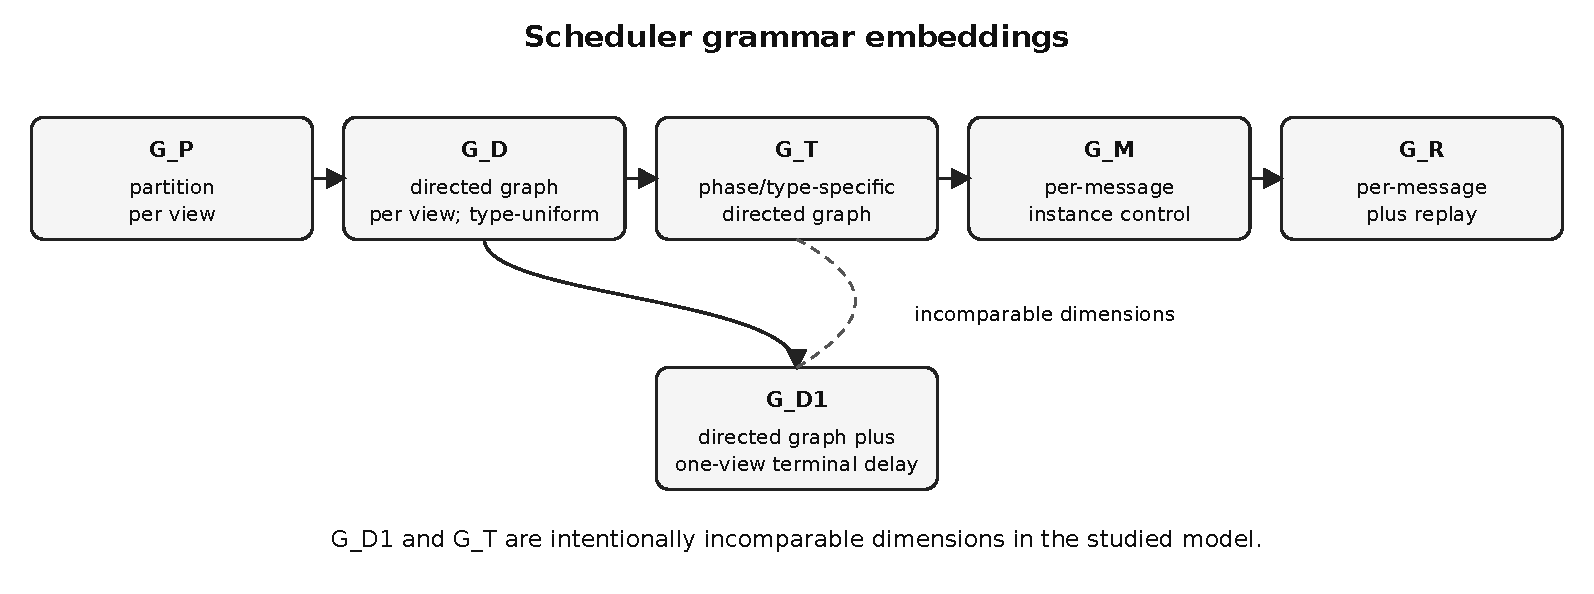
\includegraphics[width=0.92\textwidth,height=\textheight]{figures/figure1_scheduler_grammar.pdf}
\caption{Scheduler grammars and the type-erasure map. The central
comparison is between phase-specific admission and one type-uniform
directed edge bit.}
\end{figure}

\section{3. When closure preserves
unsafety}\label{when-closure-preserves-unsafety}

\subsection{3.1 Merged-trace lifting
lemma}\label{merged-trace-lifting-lemma}

Let \(R\subseteq S\times S\) be a preorder. Consider an original trace
and a merged trace that retains every original action in order and
inserts closure-required delivery actions. Suppose:

\begin{itemize}
\tightlist
\item
  \textbf{initial relation:} \(R(s_0,s_0)\);
\item
  \textbf{increasing insertion:} for every inserted action \(b\),
  \(R(s,\delta(s,b))\);
\item
  \textbf{forward simulation:} for every retained action \(a\),
  \(R(s,t)\) implies \(R(\delta(s,a),\delta(t,a))\);
\item
  \textbf{transitivity:} \(R\) is transitive.
\end{itemize}

\textbf{Lemma 1 (merged-trace lifting).} If the original and merged
traces begin in related states, then their terminal states are related.

\textbf{Proof.} Induct over the merged trace while counting how many
original actions have been consumed. At an inserted action, increasing
insertion extends the relation and transitivity composes it with the
current invariant. At a retained action, forward simulation advances
both sides. At the end, all original actions have been consumed, giving
the terminal relation. \(\square\)

\subsection{3.2 Legal scheduler-closure
theorem}\label{legal-scheduler-closure-theorem}

Assume additionally that unsafety is upward closed:

\[
R(s,t)\land\mathsf{Unsafe}(s)\Rightarrow\mathsf{Unsafe}(t).
\]

\textbf{Theorem 1 (legal relational closure preservation).} Let
\(\tau\in L_{G_T}(P,B)\) be unsafe. If the type-erasure transform
\(C(\tau)\) is a legal target execution in \(L_{G_D}(P,B)\) and the four
relational premises above hold for the inserted and retained actions of
\(C(\tau)\), then

\[
\mathsf{Unsafe}(\operatorname{last}(C(\tau))).
\]

Consequently,

\[
O(\operatorname{last}(C(\tau)))
\in \mathsf{UnsafeObs}_{G_D}(P,B).
\]

\textbf{Proof.} Target legality supplies a valid coarse execution. Lemma
1 gives \(R(\operatorname{last}(\tau),\operatorname{last}(C(\tau)))\).
Upward closure transfers unsafety to the target terminal state. Applying
\(O\) yields a member of the target unsafe-observation language.
\(\square\)

The theorem is sufficient, not necessary. It makes clear why ``more
delivered messages'' is not automatically monotone: an inserted message
may remove future behavior relevant to the safety witness, so no
suitable preorder with upward-closed unsafety exists.

\section{4. Quorum-pivot separation}\label{quorum-pivot-separation}

\subsection{4.1 Structural criterion}\label{structural-criterion}

Let \(P\) be a bounded certificate-driven locking system with threshold
\(q\). Consider two conflicting decision opportunities \(C_0<C_1\) for
values \(0\) and \(1\). The following premises define the structural
mechanism.

\begin{enumerate}
\def\labelenumi{\arabic{enumi}.}
\tightlist
\item
  Each branch has fixed base support of \(q-1\) contributions.
\item
  A correct identity \(p\) is the only contribution capable of
  completing both branches inside the bound.
\item
  An already-emitted enabling envelope \(E\) is processed before \(C_0\)
  and makes \(p\) available to the first branch.
\item
  An already-emitted repair envelope \(R\) is processed after \(C_0\)
  but before \(C_1\) and makes \(p\) unavailable to the second branch.
\item
  \(E\) and \(R\) have the same view, sender, and receiver but distinct
  phase labels.
\item
  A phase-specific policy admits \(E\) and withholds \(R\).
\item
  The directed grammar has one Boolean bit for that shared edge; all
  other productions, edges, deliveries, and phase order are fixed. Edge
  off withholds both envelopes, and edge on processes both in the order
  \(E<C_0<R<C_1\).
\item
  A correct decision for value \(i\) is emitted when the corresponding
  certificate reaches \(q\), and decisions are irreversible inside the
  bound.
\end{enumerate}

\textbf{Theorem 2 (quorum-pivot separation criterion).} Every bounded
system satisfying Premises 1--8 has an agreement-violating execution
under \(G_T\), while no execution in the stated \(G_D\) domain violates
agreement:

\[
\mathsf{UnsafeObs}_{G_T}(P,B)\neq\varnothing,
\qquad
\mathsf{UnsafeObs}_{G_D}(P,B)=\varnothing.
\]

\textbf{Proof.} Under \(G_T\), \(E\) is delivered and \(R\) is not. The
first base of \(q-1\) plus \(p\) forms the value-0 certificate and
decision at \(C_0\). Since repair is absent, \(p\) remains available;
the second base plus \(p\) forms the conflicting value-1 certificate and
decision at \(C_1\).

For \(G_D\), the Boolean domain is exhaustive. If the edge is off,
neither \(E\) nor \(R\) is delivered, so the first branch remains at
\(q-1\). If the edge is on, \(E\) enables the first certificate, but
\(R\) is processed before \(C_1\) and disables \(p\); the second branch
remains at \(q-1\). Hence neither directed execution contains two
conflicting correct decisions. \(\square\)

This theorem is the intermediate structural result: it identifies a
checkable mechanism without tying the statement to one hand-written
quorum arithmetic instance.

\subsection{\texorpdfstring{4.2 Parametric \(3f+1\)
family}{4.2 Parametric 3f+1 family}}\label{parametric-3f1-family}

For every \(f\geq1\), let

\[
n=3f+1,\qquad q=2f+1.
\]

Partition identities into \(B,A,C,\) and \(\{p\}\), with

\[
|B|=|A|=|C|=f,
\]

where \(B\) is Byzantine, \(A\) supports only value \(0\), \(C\)
supports only value \(1\), and \(p\) is correct. Define

\[
Q_0=B\cup A\cup\{p\},
\qquad
Q_1=B\cup C\cup\{p\}.
\]

Then \(|Q_0|=|Q_1|=2f+1=q\), while each branch without \(p\) has
\(2f=q-1\) contributions. The correct intersection of the two quorums is
exactly \(\{p\}\).

The bounded domain \(B_f\) fixes one pair of conflicting values, one
shared controlled edge, the order \(E<C_0<R<C_1\), all other messages
and edges, once-only delivery, and the absence of late repair after
\(C_1\). The only \(G_D\) degree of freedom is the Boolean edge bit. Let
\(P_f\) be the protocol schema with the decisions specified in Premise
8.

\textbf{Corollary 1 (parametric family).} For every \(f\geq1\),

\[
\mathsf{UnsafeObs}_{G_D}(P_f,B_f)=\varnothing,
\qquad
\mathsf{UnsafeObs}_{G_T}(P_f,B_f)\neq\varnothing.
\]

The arithmetic is immediate from \(2f+1=q\) and \(2f=q-1\); the
behavioral result follows from Theorem 2.

\begin{figure}
\centering
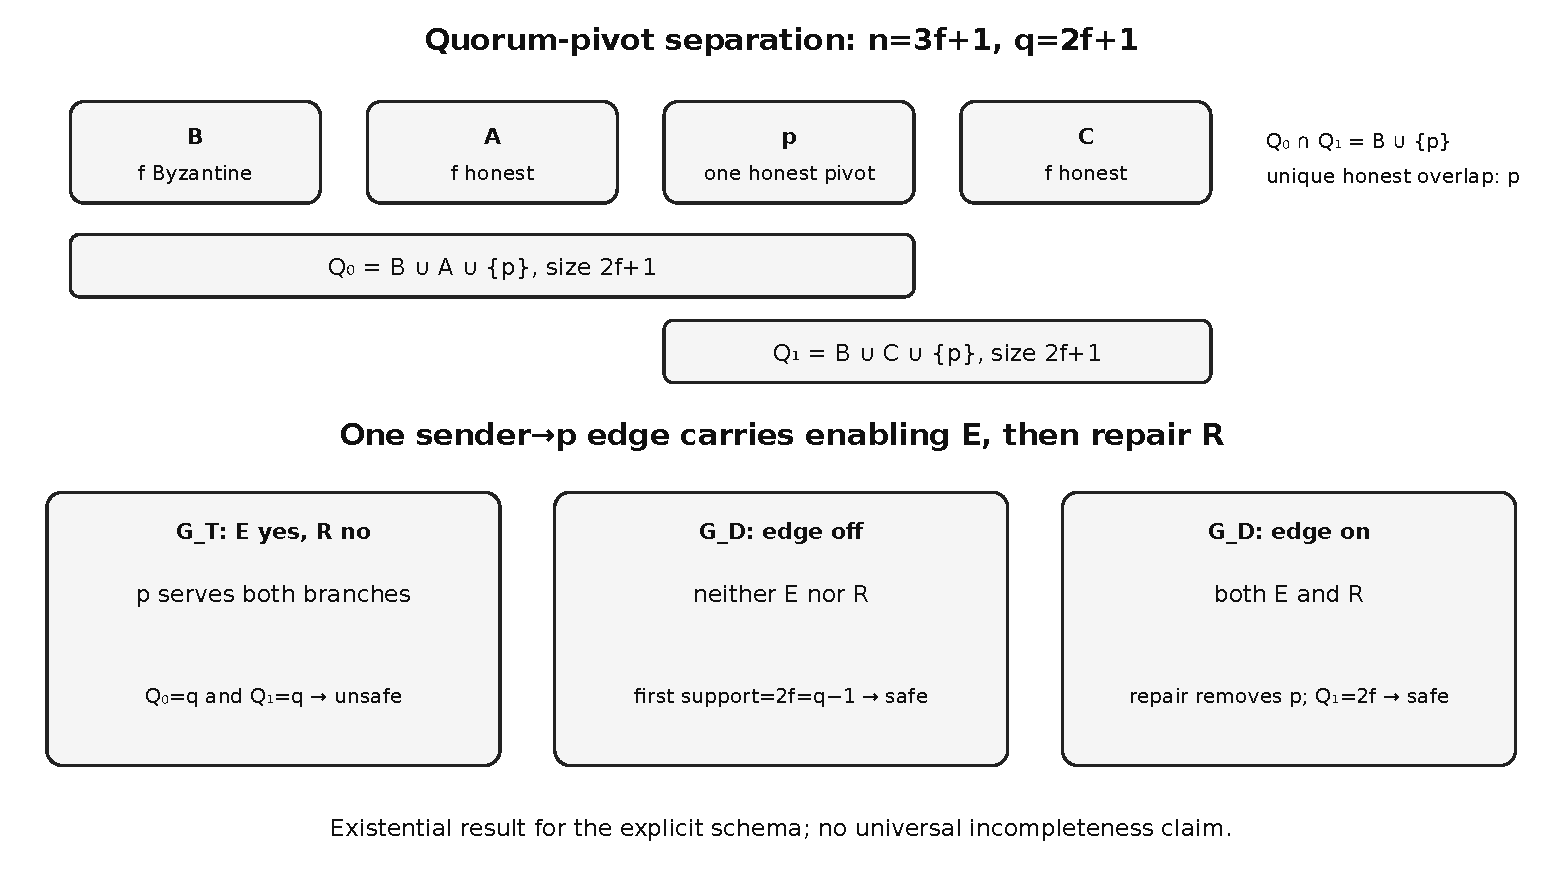
\includegraphics[width=0.94\textwidth,height=\textheight]{figures/figure2_quorum_pivot.pdf}
\caption{Quorum-pivot mechanism. The fine policy admits enabling
evidence but withholds repair; the closed policy either loses the first
quorum or repairs the pivot before the second.}
\end{figure}

\section{5. Diagnostic seven-premise
boundary}\label{diagnostic-seven-premise-boundary}

The structural theorem uses semantic premises. For bounded diagnosis and
ablation, we encode seven Boolean flags:

\begin{itemize}
\tightlist
\item
  \(S_1\): the first base is one short of quorum;
\item
  \(S_2\): the second base is one short of quorum;
\item
  \(R_q\): the pivot's second-branch participation requires enabling
  evidence;
\item
  \(D\): repair disables the pivot;
\item
  \(T\): repair is processed before the second opportunity;
\item
  \(E_d\): enabling and repair share the endpoint/view erased by
  closure;
\item
  \(X\): the fine grammar can distinguish their phase labels.
\end{itemize}

For delivery bits \(e\) and \(r\), the operational unsafe outcome is

\[
U(e,r)=
(\neg S_1\lor e)
\land
\left[
\neg S_2
\lor
\left((\neg R_q\lor e)\land
\neg(r\land D\land T)
\right)
\right].
\]

Strict separation is

\[
\mathsf{Strict}
=
X\land E_d\land
U(1,0)\land
\neg U(0,0)\land
\neg U(1,1).
\]

\textbf{Proposition 1 (exact boundary of the diagnostic abstraction).}
Over all \(2^7\) assignments,

\[
\mathsf{Strict}
\iff
S_2\land D\land T\land E_d\land X\land(S_1\lor R_q).
\]

\textbf{Derivation.} Direct substitution gives

\[
U(1,0)=\mathsf{true},
\]

\[
U(0,0)=\neg S_1\land(\neg S_2\lor\neg R_q),
\]

and

\[
U(1,1)=\neg S_2\lor\neg D\lor\neg T.
\]

Therefore

\[
\neg U(0,0)=S_1\lor(S_2\land R_q),
\]

\[
\neg U(1,1)=S_2\land D\land T.
\]

Conjoining with \(X\land E_d\) and simplifying under \(S_2\) yields

\[
X\land E_d\land S_2\land D\land T\land(S_1\lor R_q).
\]

In the flag order \((S_1,S_2,R_q,D,T,E_d,X)\), the satisfying
assignments are exactly

\begin{verbatim}
0111111
1101111
1111111
\end{verbatim}

The exhaustive truth table is a cross-check of this algebra, not the
proof's conceptual core. Proposition 1 characterizes only this
seven-flag operational abstraction; it is not a necessary-and-sufficient
theorem for all locking protocols.

\begin{figure}
\centering
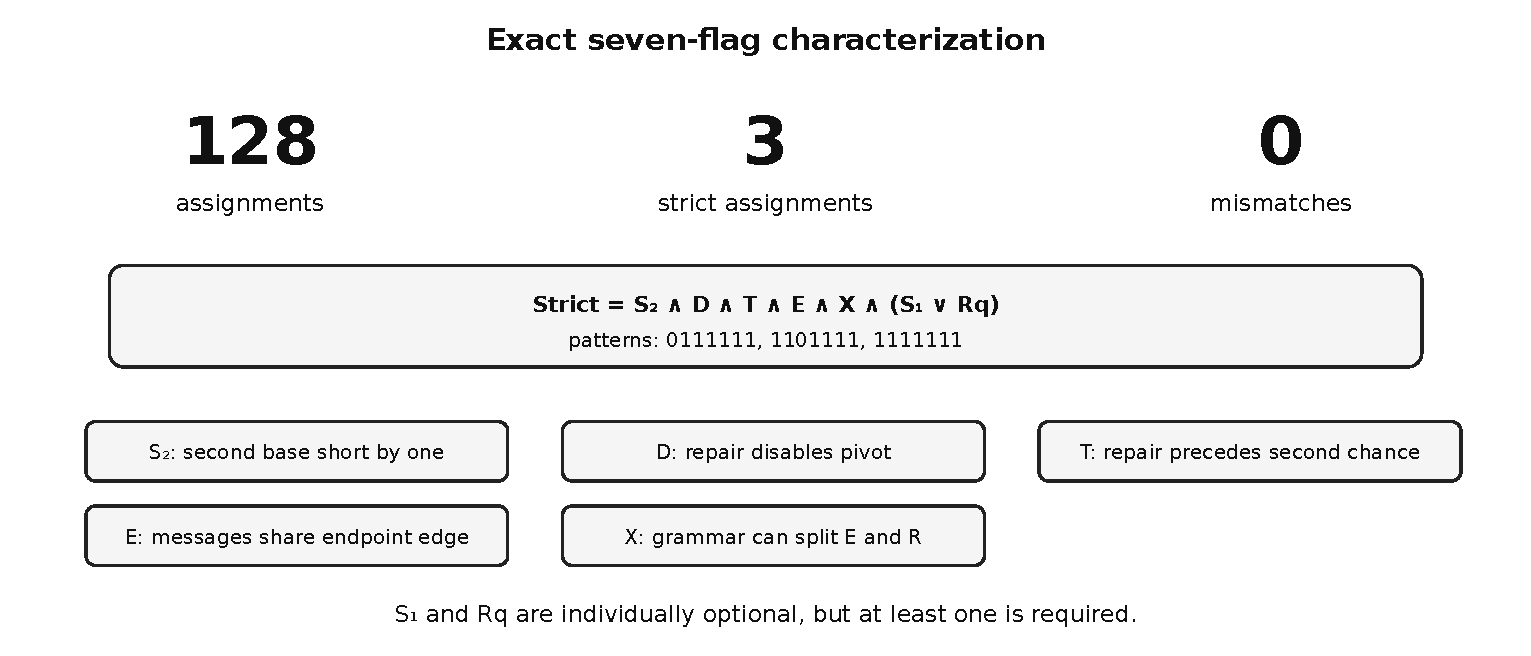
\includegraphics[width=0.9\textwidth,height=\textheight]{figures/figure3_premise_boundary.pdf}
\caption{The diagnostic premise boundary. Five premises are always
necessary; at least one of first-branch shortage or enabling-dependent
reuse must hold.}
\end{figure}

\section{6. Bounded instantiation to Tendermint-style
locking}\label{bounded-instantiation-to-tendermint-style-locking}

\subsection{6.1 Published rule
vocabulary}\label{published-rule-vocabulary}

The CometBFT consensus specification organizes each round as
\texttt{Propose}, \texttt{Prevote}, and \texttt{Precommit}, followed by
\texttt{Commit} once a block receives more than two-thirds precommits. A
more-than-two-thirds prevote set for a block is a
proof-of-lock-change/PoLC; in the normal rule, a validator seeing such
evidence locks or relocks the block and precommits it (CometBFT Project
2026). We use these published rules as a natural transition vocabulary,
not as evidence of an implementation bug.

The bounded instance fixes one height \(H\), rounds \(r_0=0\) and
\(r_1=1\), values \(0\) and \(1\), and the same \(3f+1\) validator
partition as Section 4. The controlled mutation is
\texttt{MISSING\_LOCK\_UPDATE}: after observing a round-0 PoLC for value
\(0\), the pivot emits \texttt{PRECOMMIT(0,H,r\_0)} but fails to persist
\texttt{lockedValue=0} and \texttt{lockedRound=r\_0}.

\subsection{6.2 Refinement map}\label{refinement-map}

\begin{longtable}[]{@{}
  >{\raggedright\arraybackslash}p{(\columnwidth - 2\tabcolsep) * \real{0.5000}}
  >{\raggedright\arraybackslash}p{(\columnwidth - 2\tabcolsep) * \real{0.5000}}@{}}
\toprule\noalign{}
\begin{minipage}[b]{\linewidth}\raggedright
Abstract object
\end{minipage} & \begin{minipage}[b]{\linewidth}\raggedright
Bounded Tendermint-style rule
\end{minipage} \\
\midrule\noalign{}
\endhead
\bottomrule\noalign{}
\endlastfoot
pivot \(p\) & correct validator required by both conflicting \(2f+1\)
precommit sets \\
enabling \(E\) & last \texttt{PREVOTE(0,H,r0)} from fixed Byzantine
sender \(b_0\) to \(p\), completing \(p\)'s local PoLC \\
first opportunity \(C_0\) & a correct observer receives
\(B\cup A\cup\{p\}\) precommits and decides value \(0\) \\
repair \(R\) & last \texttt{PRECOMMIT(0,H,r0)} from the same \(b_0\) to
\(p\), completing \(p\)'s local commit set \\
disabled pivot & baseline lock prevents conflicting precommit, or
receipt of \(R\) makes \(p\) commit/advance before \(C_1\) \\
second opportunity \(C_1\) & later round-1 value-1 precommit set
\(B\cup C\cup\{p\}\) \\
shared edge & same \(H,r_0,b_0,p\); labels differ only as
\texttt{PREVOTE} versus \texttt{PRECOMMIT} \\
\end{longtable}

The bound fixes every other message, edge, and delivery. It processes
the events in the order

\[
E < C_0 < R < C_1.
\]

There is no late delivery of \(R\) after \(C_1\). Thus the type-uniform
directed domain has exactly two policies: edge off and edge on. The
phase-specific witness admits \(E\) and rejects \(R\).

\subsection{6.3 Result}\label{result}

\textbf{Proposition 2 (bounded Tendermint-style instantiation).} For
every \(f\geq1\) in the supplied rule-level model:

\begin{itemize}
\tightlist
\item
  the unmutated locking rule is safe under the phase-specific witness
  and both directed policies;
\item
  under \texttt{MISSING\_LOCK\_UPDATE}, the phase-specific policy yields
  conflicting correct decisions;
\item
  under the same mutation, both directed policies remain safe.
\end{itemize}

The proof is a direct refinement to Theorem 2. With edge off, \(p\)
never sees the PoLC-completing prevote, so the value-0 certificate is
short. With edge on, \(p\) sees both the enabling prevote and the
commit-completing precommit; the latter is processed before the value-1
opportunity and removes \(p\) from the second branch. Under
phase-specific admission, the mutation leaves \(p\) unlocked and
uncommitted after the first branch, permitting the conflicting
contribution.

Two independent implementations enumerate the bounded rule system.
Python and Go produce identical terminal rows for six combinations of
baseline/mutant and scheduler policy for each \(f=1,\ldots,64\), for 384
cases per implementation. An additional independent checker evaluates
the same semantic conditions through \(f=128\). These executions
validate the stated refinement; they do not establish conformance of the
entire production event loop or the existence of the mutation in
CometBFT.

\section{7. Replay erasure as a secondary closure
dimension}\label{replay-erasure-as-a-secondary-closure-dimension}

Phase erasure is the main result. Replay illustrates a different
boundary: a repeated byte string may be immediately silent yet alter
hidden state that affects future processing.

Let \(\pi:S\to S_{\mathrm{rel}}\) project protocol-relevant state,
including the set of processed stable message keys. Let
\(\delta:S\times M\to S\) be the transition function and

\[
\mathsf{out}:S\times M\to O^*
\]

the protocol-relevant output produced while processing one message.

We require two congruence conditions for every message \(m\):

\[
\pi(s)=\pi(t)
\Rightarrow
\pi(\delta(s,m))=\pi(\delta(t,m)),
\tag{state congruence}
\]

and

\[
\pi(s)=\pi(t)
\Rightarrow
\mathsf{out}(s,m)=\mathsf{out}(t,m).
\tag{output congruence}
\]

For a marked duplicate whose stable key is already represented in
\(\pi(s)\), require

\[
\pi(\delta(s,m))=\pi(s)
\quad\text{and}\quad
\mathsf{out}(s,m)=\epsilon.
\]

\textbf{Theorem 3 (replay erasure with outputs).} Under state
congruence, output congruence, projected duplicate stutter, and
duplicate output silence, erasing all marked duplicates from a finite
trace preserves both the final relevant projection and the entire
protocol-relevant output trace. Any state-based observation that factors
through \(\pi\) is therefore preserved.

\textbf{Proof.} Induct over the original trace and its erased trace
while maintaining equality of current projections and accumulated
relevant outputs. A marked duplicate leaves the full execution's
projection unchanged and appends no output, so the erased side may
stutter. For a retained message, state congruence preserves equality of
the next projections and output congruence appends equal output
fragments. The terminal invariant gives both conclusions. \(\square\)

The output premise is necessary for the output-trace claim. Equal
projections alone permit hidden states to emit different future outputs.
State congruence is also necessary: in the counterexample trace
\texttt{X,X,Y}, the second \texttt{X} changes only a hidden bit and
produces no output, while \texttt{Y} copies that bit into relevant
state. The full and deduplicated traces then have different
observations. The artifact includes this counterexample and a separate
output-congruence negative control.

\section{8. Evidence and formal
assurance}\label{evidence-and-formal-assurance}

\subsection{8.1 Independent finite
checks}\label{independent-finite-checks}

The final artifact includes a checker that imports neither the project
models nor the proof-certificate kernel. It verifies:

\begin{itemize}
\tightlist
\item
  exact scheduler filtering, no synthesis, once-only delivery, and
  stable order;
\item
  legal-target relational lifting over all valid two-state finite
  instances in its scope;
\item
  the structural criterion for quorum thresholds \(1\) through \(64\);
\item
  the hidden-state replay counterexample and positive state/output
  congruence cases;
\item
  the bounded Tendermint-style bridge for \(f=1\) through \(128\);
\item
  the corrected typing of \texttt{UnsafeObs}.
\end{itemize}

The post-audit SMT package contains positive obligations and damaged
controls. Z3 (Moura and Bjørner 2008) is expected to return
\texttt{UNSAT} for the preservation obligations and \texttt{SAT} for
controls that drop a necessary condition. Go exact arithmetic
independently checks the parametric quorum equations.

\subsection{8.2 Prover developments}\label{prover-developments}

The archive contains Lean and Coq sources for scheduler semantics, typed
unsafe observations, legal closure lifting, the structural criterion,
the parametric family, the Tendermint-style instantiation, replay
erasure with outputs, and the diagnostic boundary. Internal
proof-obligation identifiers appear only in the artifact map; the paper
uses normal theorem numbering.

A purpose-built certificate checker and the SMT obligations execute in
the supplied environment. The mature-prover source is pinned and
source-hygiene checked. A successful Lean or Coq kernel build remains a
release condition when the corresponding compiler is available; the
reproduction script does not convert an absent external toolchain into a
\texttt{PASS}.

\subsection{8.3 Executable validation}\label{executable-validation}

Earlier gates supply two finite locking kernels and a fuller two-round
event loop with \texttt{PROPOSAL}, \texttt{PREVOTE}, \texttt{POLKA},
\texttt{PRECOMMIT}, and \texttt{COMMIT}. The baseline is safe across the
tested grammars. Controlled obligation violations distinguish phase
control, terminal delay, and replay. A Go implementation and an
independently written Python mirror agree on canonical terminal cases,
while FIFO, LIFO, and seeded event orders preserve the safety
classifications. These results test the mechanism and implementation
correspondence inside the declared bounds; they are not a statistical
estimate of production bug prevalence.

\section{9. Related work and novelty
boundary}\label{related-work-and-novelty-boundary}

Twins uses same-identity replicas and round-indexed communication
patterns to exercise equivocation, double voting, and state loss (Bano
et al. 2022). Randomized BFT testing provides message mutation and
richer fault exploration (Winter et al. 2023). Netrix and ByzzBench
provide controlled scheduling and evaluation infrastructure (Drăgoi,
Nagendra, and Srivas 2024; Neto and Ozkan 2025). ByzTwin-Range broadens
practical Byzantine experimentation through a digital-twin cyber-range
(Freitas, Soares, and Martins 2026). None of these implementation
capabilities is claimed as new here.

Communication closure is the closest conceptual result. It establishes a
property-preserving testing reduction for a class of consensus
implementations (Drăgoi et al. 2020). Our closure operator and boundary
differ: phase labels on already-emitted messages are erased to one
endpoint bit, and closure-added repair can remove the only correct
contribution shared by two conflicting quorum opportunities. Heard-Of
and closed message-adversary work already provide directed per-round
communication semantics (Charron-Bost and Schiper 2009; Winkler, Schmid,
and Moses 2020), so the graph model itself is not a contribution.

VLSM develops formal validator-system traces and Byzantine/equivocation
relationships under validity assumptions (Barreto et al. 2022).
Functional reasoning for distributed systems connects restricted
synchronous reasoning to asynchronous operational semantics in Rocq (Ni,
Renesse, and Morrisett 2025). These works motivate explicit
legal-language and refinement obligations. PERF formalizes fault
injectors and composition for performance prediction (Zhou et al. 2026),
which further rules out a novelty claim based on injector taxonomies.

\begin{table}[t]
\centering
\scriptsize
\setlength{\tabcolsep}{2.5pt}
\begin{tabular}{lccccccc}
\toprule
Work & Part. & Dir. & Phase & Inst. & Replay & Closure & Sep.\\
\midrule
Twins & Y & part. & -- & -- & state & -- & --\\
Comm. closure & -- & lossy & -- & -- & -- & Y & --\\
HO/msg. adv. & -- & Y & -- & -- & -- & sem. & --\\
Rand. BFT test & -- & Y & Y & Y & Y & -- & --\\
Netrix & -- & Y & Y & Y & Y & -- & --\\
ByzzBench & cfg. & Y & cfg. & cfg. & cfg. & -- & --\\
PERF & -- & model & faults & model & model & perf. & --\\
\textbf{This work} & case & Y & Y & formal & Y & \textbf{Y} & \textbf{Y}\\
\bottomrule
\end{tabular}
\caption{Capability map for closest work. `Closure' denotes an explicit property-preservation result; `Sep.' denotes a safety-observation separation witness.}
\end{table}

The table is a capability map, not a quality ranking. The novelty claim
is search-bounded: in sources reviewed through 21 August 2026, we found
no result combining the same phase-erasure closure, legal-target
condition, finite agreement projection, repair/unique-pivot criterion,
bounded Tendermint-style refinement, exact diagnostic boundary, and
replay theorem with both state and output congruence. Absolute novelty
is not asserted.

\section{10. Validity and limitations}\label{validity-and-limitations}

\textbf{Internal validity.} A shared specification error could affect
the formal and executable routes. Mitigations include independent Python
and Go models, an independent checker, SMT encodings with damaged
controls, exact arithmetic, source-level prover developments, and a safe
unmutated baseline. The natural protocol bridge is deliberately small
enough to inspect line by line.

\textbf{Construct validity.} Scheduler expressiveness is measured by the
set of unsafe terminal observations, not schedule count, code coverage,
or bug yield. A different property can induce a different grammar
ordering. Type closure is precisely the stable-filter operator of
Section 2; systems that permit delay inside a view, phase-specific
exceptions, or delivery outside partitions need a separate conformance
map.

\textbf{External validity.} The family uses unweighted \(3f+1\) quorums
and finite views. The Tendermint-style bridge is rule-level and bounded.
Weighted stake, validator-set changes, multi-height state transfer, disk
recovery, liveness, and pacemaker behavior are outside the theorem. The
bridge does not show that CometBFT contains
\texttt{MISSING\_LOCK\_UPDATE}.

\textbf{Proof assurance.} The mathematical obligations are independently
encoded and checked in several routes, but only an executed
mature-prover build can remove the remaining compiler-level assurance
condition for the Lean/Coq sources. The artifact reports that status
explicitly.

\textbf{Responsible use.} All adversarial schedules and mutations run
locally. No public network, assets, private keys, denial-of-service
traffic, or unauthorized access are involved. A future
implementation-level finding should be privately minimized and disclosed
before publication of sensitive details.

\section{11. Reproducibility}\label{reproducibility}

The artifact exposes one entry point:

\begin{verbatim}
./reproduce.sh
\end{verbatim}

It runs the independent proof checks, the Python and Go Tendermint-style
bridge, cross-language comparison, project-local certificate checks, SMT
obligations, tests, source hygiene, and manuscript/PDF checks. The final
summary prints a separate line for each theorem package and for negative
controls. If Lean or Coq is installed, the same entry point builds the
pinned project and runs the axiom audit; otherwise it records the
mature-prover step as unavailable rather than silently skipping it.

The package preserves raw and processed outputs, fixed random seeds,
protocol parameters, source registers, tool versions, and SHA-256
manifests. Historical research gates are included under
\texttt{historical/}, while the final paper, formal sources, protocol
instantiation, and current evidence occupy the top-level project.

\section{12. Conclusion}\label{conclusion}

Phase erasure can change more than the number of schedules. When
enabling and repair evidence share one endpoint and view, but differ by
phase, closing their admission to a single directed edge bit can insert
repair before a later certificate opportunity. If repair disables the
unique correct quorum pivot, the coarse grammar deletes an
agreement-violation witness.

A legal relational theorem identifies when closure is safe; a structural
criterion identifies when the locking mechanism defeats that
monotonicity; the \(3f+1\) family and bounded Tendermint-style
instantiation make the boundary concrete. The diagnostic seven-premise
model states the exact local conditions, while the replay theorem shows
why future state and output congruence are required for duplicate
erasure.

The practical implication is methodological. Testing frameworks should
not equate a richer API with a scientific result, nor interpret a
smaller scheduler language as property preserving without a closure
proof. For a concrete protocol, one must either discharge the legal and
relational obligations or exhibit a minimal separation witness and name
the missing premise.

\section{Acknowledgment and AI-use disclosure
draft}\label{acknowledgment-and-ai-use-disclosure-draft}

The anonymous draft was prepared with substantial assistance from an
OpenAI language model for research organization, source discovery, prose
drafting, code and artifact generation, and consistency checking. Human
authors must independently verify every proof, citation, experiment, and
source and remain fully accountable for the manuscript. The model is not
an author. This statement must be adapted to the final venue policy.

\section*{References}\label{references}
\addcontentsline{toc}{section}{References}

\phantomsection\label{refs}
\begin{CSLReferences}{1}{0}
\bibitem[\citeproctext]{ref-bano2021twins}
Bano, Shehar, Alberto Sonnino, Andrey Chursin, Dmitri Perelman, Zekun
Li, Avery Ching, and Dahlia Malkhi. 2022. {``Twins: {BFT} Systems Made
Robust.''} In \emph{25th International Conference on Principles of
Distributed Systems (OPODIS 2021)}, 217:7:1--29. Leibniz International
Proceedings in Informatics (LIPIcs).
\url{https://doi.org/10.4230/LIPIcs.OPODIS.2021.7}.

\bibitem[\citeproctext]{ref-barreto2022vlsm}
Barreto, Miguel et al. 2022. {``Validating Labelled State and Message
Production Systems.''} \emph{arXiv Preprint arXiv:2202.12662}.
\url{https://arxiv.org/abs/2202.12662}.

\bibitem[\citeproctext]{ref-charronbost2009heardof}
Charron-Bost, Bernadette, and André Schiper. 2009. {``The Heard-of
Model: Computing in Distributed Systems with Benign Faults.''}
\emph{Distributed Computing} 22 (1): 49--71.
\url{https://doi.org/10.1007/s00446-009-0084-6}.

\bibitem[\citeproctext]{ref-cometbft0393}
CometBFT Project. 2026. {``CometBFT Consensus Specification.''} Release
v0.39.3, commit prefix 49b8283.
\url{https://github.com/cometbft/cometbft/blob/v0.39.3/spec/consensus/consensus.md}.

\bibitem[\citeproctext]{ref-dragoi2020communication}
Drăgoi, Cezara, Constantin Enea, Burcu Kulahcioglu Ozkan, Rupak
Majumdar, and Filip Nikšić. 2020. {``Testing Consensus Implementations
Using Communication Closure.''} \emph{Proceedings of the ACM on
Programming Languages} 4 (OOPSLA): 210:1--29.
\url{https://doi.org/10.1145/3428278}.

\bibitem[\citeproctext]{ref-dragoi2024netrix}
Drăgoi, Cezara, Srinidhi Nagendra, and Mandayam Srivas. 2024. {``A
Domain Specific Language for Testing Distributed Protocol
Implementations.''} In \emph{Networked Systems (NETYS 2024)}, 100--117.
Lecture Notes in Computer Science.
\url{https://doi.org/10.1007/978-3-031-67321-4_6}.

\bibitem[\citeproctext]{ref-freitas2026byztwin}
Freitas, Tadeu, João Soares, and Rolando Martins. 2026. {``Trust, but
Verify: ByzTwin-Range, a Digital Twin Cyber-Range for Byzantine
Faults.''} \emph{arXiv Preprint arXiv:2604.18049}.
\url{https://arxiv.org/abs/2604.18049}.

\bibitem[\citeproctext]{ref-moura2008z3}
Moura, Leonardo de, and Nikolaj Bjørner. 2008. {``Z3: An Efficient SMT
Solver.''} In \emph{Tools and Algorithms for the Construction and
Analysis of Systems (TACAS 2008)}, 4963:337--40. Lecture Notes in
Computer Science. \url{https://doi.org/10.1007/978-3-540-78800-3_24}.

\bibitem[\citeproctext]{ref-louroneto2025byzzbench}
Neto, João Miguel Louro, and Burcu Kulahcioglu Ozkan. 2025. {``A
Benchmark Framework for Byzantine Fault Tolerance Testing Algorithms.''}
In \emph{6th International Workshop on Formal Methods for Blockchains
(FMBC 2025)}, 129:13:1--11. Open Access Series in Informatics (OASIcs).
\url{https://doi.org/10.4230/OASIcs.FMBC.2025.13}.

\bibitem[\citeproctext]{ref-ni2025functional}
Ni, Haobin, Robbert van Renesse, and Greg Morrisett. 2025. {``Functional
Reasoning for Distributed Systems with Failures.''} \emph{arXiv Preprint
arXiv:2510.12131}. \url{https://arxiv.org/abs/2510.12131}.

\bibitem[\citeproctext]{ref-winkler2020closed}
Winkler, Kyrill, Ulrich Schmid, and Yoram Moses. 2020. {``A
Characterization of Consensus Solvability for Closed Message
Adversaries.''} In \emph{23rd International Conference on Principles of
Distributed Systems (OPODIS 2019)}, 153:17:1--16. Leibniz International
Proceedings in Informatics (LIPIcs).
\url{https://doi.org/10.4230/LIPIcs.OPODIS.2019.17}.

\bibitem[\citeproctext]{ref-winter2023randomized}
Winter, Levin N., Florena Buşe, Daan de Graaf, Klaus von Gleissenthall,
and Burcu Kulahcioglu Ozkan. 2023. {``Randomized Testing of Byzantine
Fault Tolerant Algorithms.''} \emph{Proceedings of the ACM on
Programming Languages} 7 (OOPSLA1): 757--88.
\url{https://doi.org/10.1145/3586053}.

\bibitem[\citeproctext]{ref-zhou2026perf}
Zhou, Ziwei, Si Liu, Zhou Zhou, Peixin Wang, and Min Zhang. 2026. {``A
Formal Framework for Predicting Distributed System Performance Under
Faults.''} \emph{arXiv Preprint arXiv:2602.19088}.
\url{https://arxiv.org/abs/2602.19088}.

\end{CSLReferences}

\end{document}
